\documentclass[conference]{IEEEtran}

% Paquets necessaris
\usepackage{graphicx} % Per incloure imatges
\usepackage{courier}
\usepackage[catalan]{babel} % Per usar el català
\usepackage{multicol}
\usepackage{multirow}
\usepackage{titlesec}
\usepackage{dsfont}
\usepackage{pgffor}
\usepackage{amsfonts}
\usepackage{algorithm}
\usepackage{algpseudocode}
\usepackage[x11names]{xcolor}
\usepackage[colorlinks = true,
            linkcolor = blue,
            urlcolor  = blue,
            citecolor = blue,
            anchorcolor = blue]{hyperref}%hiperenllaços

% Configuración de las columnas
\setlength{\columnsep}{0.2 in} % Separación entre columnas
\setlength{\columnwidth}{3.5 in} % Ancho de cada columna

\titleformat{\subsubsection}
  {\normalfont\bfseries\large}{\thesubsubsection}{1em}{\quad}
\renewcommand\thesubsubsection{\thesubsection.\arabic{subsubsection}}




% Cambiar el formato de numeración de las secciones
\renewcommand{\thesection}{\arabic{section}}
\renewcommand{\thesubsection}{\thesection.\arabic{subsection}}
\newcommand\colorrulemix[1]{\textcolor{#1!40!gray}{\rule{1cm}{1cm}} }
\newcommand\colorrule[1]{\textcolor{#1}{\rule{1cm}{1cm}} }

\titleformat{\section}{\normalfont\Large\bfseries}{\thesection}{1em}{}
\titleformat{\subsection}{\normalfont\large\bfseries}{\thesection.\arabic{subsection}}{1em}{}

\pagestyle{plain}
\pagenumbering{arabic}


% Información del documento
\title{Pràctica 5: Diferenciador d'Idiomes}
\author{Jaume Adrover Fernandez, Diego Bermejo Cabañas i Joan Balaguer Llagostera}

\begin{document}
\maketitle

\begin{abstract}
    En aquest document s'explicarà el contingut de la pràctica 5 sobre trobar la distància mitjana d'edició de Levenstein entre dos o més idiomes determinats. Explicarem com hem afrontat el problema, quines solucions hem implementat,  el codi desenvolupat i finalment unes conclusions amb els problemes que ens hem trobat i algunes reflexions que hem fet.
\end{abstract}

% Introducción
\section{Introducció}
En aquest article explicarem el funcionament i la implementació de la nostra pràctica, estructurant el document de tal forma que es cobreixi la totalitat de aspectes rellevants d'aquesta.\\\\
Per una part explicarem l'estructura del MVC que hem relitzat i mostrarem analíticament com funciona aquesta estructura durant l'execució del programa.\\\\
A continuació, explicarem breument el problema que ens han proposat resoldre. Mostrarem analíticament les dues solucions que hem implementat per resoldre el problema, juntament amb explicacions en pseudocodi perquè posteriorment es pugui entendre millor el codi que hem implementat\\\\
Després, mostrarem el codi implemementat per a resoldre el problema tal i com l'hem explicat a l'apartat anterior.\\\\
Finalment, explicarem com funciona la nostra aplicació una vegada s'executa, a més del problemes que ens hem trobat i com els hem acabat resolguent.\\
\section{Implementació del MVC}
Una estructura MVC (Model Vista Controlador), consta de 3 grans parts:
\begin{itemize}
  \item \textbf{Model}: és l'encarregat d'emmagatzemar les dades del programa.\\
  \item \textbf{Vista}: s'encarrega de mostrar la interfície d'usuari amb les dades del model.\\
  \item \textbf{Controlador}: encarregat de notificar canvis de la vista entre el programa principal i el model de dades.\\
\end{itemize}
 Una vegada sabem el que simbolitza cada part de l'estructura, podem entrar més en detall en el que fa cada una d'aquestes a la nostra pràctica. Per entendre-ho millor, exemplificarem el paper que jugarà cada una de les parts quan executem el programa.

 \begin{itemize}
    \item Una vegada es posa en marxa el programa principal, podem observar dos components que ens deixen escollir els idiomes a comparar. A l'esquerra tenim la llista dels idiomes implementats i a la dreta, similar però amb l'opció de "tots" afegida.\\

    \item Escollim dues opcions i posteriorment, clicam al checkbox si volem utilitzar la versió optimitzada.Aquest checkbox activarà la utilització d'un algoritme més ràpid enlloc del tradicional tots amb tots.\\

    \item Una vegada seleccionats tots els idiomes i configuració desitjada, clicam el botó de calcula. El programa principal és avisat mitjançant la vista i el controlador s'encarrega de tota la gestió de les accions.\\

    \item Quan el controlador és avisat, aquest comprova si primer hem de comprovar un amb tots o si només son dos idiomes. A continuació, miram si el model té marcada la opció d'utilitzar l'algoritme optimitzat i, finalment, executam els càlculs.\\

    \item En darrer lloc, observarem que a la finestra s'escriu el resultat en una etiqueta. Per a poder seguir utilitzant la aplicació, torneu al principi d'aquesta llista i seguiu la mateixa metodologia.\\

\end{itemize}

\begin{figure}[ht]
    \centering
    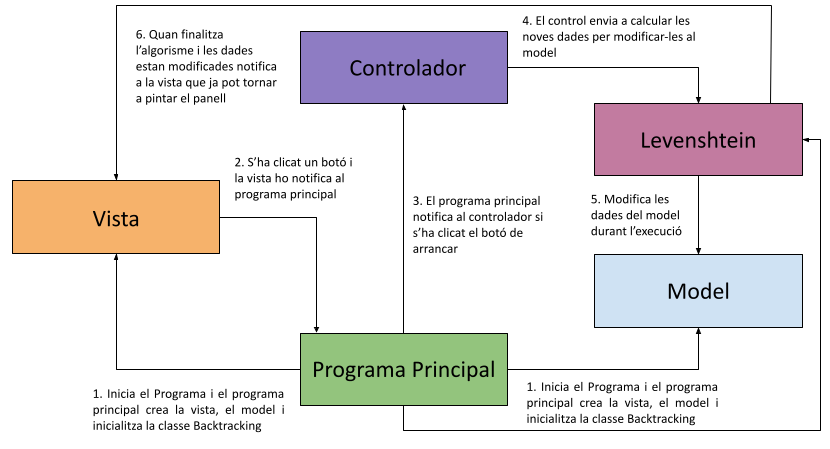
\includegraphics[width=0.388\textwidth]{images/MVC.png}
    \caption{Esquema de com funciona el nostra MVC}
\end{figure}

%3.IMPLEMENTACIÓ DE LA SOLUCIÓ
\section{Implementació de la solució}

\subsection{Problemes a resoldre}
    Durant el desenvolupament d'aquesta pràctica, hem tingut diferents inconvenients/dubtes. Vegeu la llista:

    \begin{itemize}
        \item \textbf{Qualitat de les Dades}: un dels principals problemes que ens varem trobar va ser amb la qualitat de les dades trobades. Molts de diccionaris eren amb formats extranys i depenien del país. En resum, la qualitat de la informació no era gaire bóna.


        \item \textbf{Optimització de l'algoritme}: enteníem la manera d'optimitzar, però no teníem molt clar com ordenar les paraules per longitud, a més d'obtenir els indexos de les localitzacions de les paraules segons la seva longitud.

        \item \textbf{Problema DARRER}: .
        \\
    \end{itemize}
    \subsection{Solucions adoptades}

        \begin{itemize}
            %Redacció arxiu .ltim
            \item \textbf{Manipulació de les Dades}: per a tenir unes dades de qualitat, primer de tot, vàrem haver de canviar la codificació a \textit{UTF-8}.Posteriorment, vàrem convertir tot a minúscules amb l'aplicació \textit{Notepad++}. Això vendria a ser els requisits mínims per a la compatibilitat amb la nostra versió de Java, però hem d'afegir aquests si volem utilitzar l'algoritme optimitzat:

            \begin{itemize}
                \item \textbf{Ordenació per longitud}:

                \item \textbf{Emmagatzematge indexos segons la longitud}:
            \end{itemize}

            Totes aquestes manipulacions s'han aconseguit amb un script de Python, ja que ens resultava més senzill. Vegeu-lo:\\

                %ALGORITME PYTHON
                \begin{algorithm}
                    \caption{Ordenació diccionari i generació metadata}
                    \begin{algorithmic}[1]
                        \State $dicts  \gets llistaNomsDiccionaris$
                        \State $dicts2 \gets llistaNomsDictsOrdenats$\\

                    \For{$\textrm{dict}$ \textbf{in} $\textrm{dicts}$}
                                \State $i\gets 0$
                                \For{$\textrm{word}$ \textbf{in} $\textrm{dict}$}
                                    \State $words[i]\gets word$
                                    \State $i=i+1$
                                \EndFor
                                \State $sorted\_words \gets words.ordena()$
                                \State $fWrite \gets dict+str(\_sorted.txt)$
                                \State fWrite.write(sorted\_words)
                    \EndFor\\\\

                    \For{$\textrm{dict}$ \textbf{in} $\textrm{dicts2}$}
                        \State $indexos \gets \{ \}$
                        \State $pos\gets  0$
                        \State $idx \gets 1$
                        \State $f \gets open(dict)$
                        \State $line \gets dict.readline()$
                        \While{$\textrm{line}$}
                            \State $\textrm{lon} \gets \textrm{len(line) - 1}$
                            \If{$\textrm{lon} == \textrm{idx}$}
                                \State $pos \gets pos+1$
                            \Else
                                \State $idx \gets idx+1$
                                \State $indexos[idx]=pos$
                                \State $pos \gets pos+1$
                            \EndIf
                            \State $\textrm{line} \gets f.\textrm{readline}()$
                        \EndWhile
                        \State $fitxerOut \gets dict+str(\_metadata.txt)$
                        \State $fitxerOut.write(indexos)$
                    \EndFor
                    \end{algorithmic}
                \end{algorithm}

            En resum el que es fa a l'algoritme de python és el següent:

            \begin{itemize}
                \item \textbf{Lectura de fitxers i ordenació(línies 4-13)}: com podem observar, es van afegint les paraules a un vector i després s'escriu tot a un fitxer, per exemple \textit{CAT\_sorted.txt}, que correspon al català ordenat.\\
                \item \textbf{Lectura de fitxers ordenats i metadata(línies 16-35}: en aquest bucle, el que anam fent és llegir els diccionaris ordenats i mitjançant un diccionari anotam a partir de quina posició comencen les paraules d'aquesta longitud. El diccionari segueix aquest format:
                $$dict=\{x_{0}:y_{0},x_{1}:y_{1},...,x_{n}:y_{n}|x_i \in [L_0,L_n]\}$$

                D'aquesta manera, sabem que $x_i$ pertany al conjunt de longitud possibles de les paraules d'un idioma ($L_i$). Per l'altre lloc $y_i$ correspon a l'índex corresponent on comencen les paraules de $x_i$ longitud.\\ Per exemple: \\

                $$dict=\{1:0,2:24,3:56,...\}$$

                En aquest vector, les paraules amb longitud 3 comencen a la posició 56.
            \end{itemize}

        \end{itemize}


    \subsection{Resolució general}


    %SUBSECCIÓ 3.4
    \subsection{Algoritme de Levenstein}
    Per a calcular la distància d'edició entre dues paraules, farem servir l'algorisme de Levenstein. En el nostre programa farem servir, la versió més comú d'aquest algorisme, la versió recursiva.\\

    Les diferentes operacions que es poden aplicar a una paraula per a editar-la son: reemplaçar, esborrarr i insertar.\\
    Tenint aixó en compte, poder realitzar crides recursives en les que modificam la paraula per paràmetre i incrementant el comptador del resultat. Aquest comptador ens indicará la distància resultant entre les dues paraules:
    \begin{itemize}
        \item Afegir: $return  (a_1..a_{n-1}, b_1..b_m) + 1$
        \item Esborrar: $return (a_1..a_n, b_1..b_{m-1}) + 1$
        \item Reemplaçar: $return (a_1..a_{n-1}, b_1..b_{m-1}) + 1$
    \end{itemize}

    Per a calcular la distància d'edició entre dues paraules, farem servir l'algorisme de Levenstein. En el nostre programa farem servir, la versió més comú d'aquest algorisme, la versió recursiva.\\
    
    Les diferentes operacions que es poden aplicar a una paraula per a editar-la son: reemplaçar, esborrarr i insertar.\\

    Tenint aixó en compte, poder realitzar crides recursives en les que modificam la paraula per paràmetre i incrementant el comptador del resultat. Aquest comptador ens indicará la distància resultant entre les dues paraules:
    \begin{itemize}
        \item Afegir: $return  (a_1..a_{n-1}, b_1..b_m) + 1$
        \item Esborrar: $return (a_1..a_n, b_1..b_{m-1}) + 1$
        \item Reemplaçar: $return (a_1..a_{n-1}, b_1..b_{m-1}) + 1$
    \end{itemize}
    Farem aquestes crides recursives fins a arribar a un cas base en el que una de les dues paraules queda buida. En aquest cas haurem de retornar la longitud de l'altra paraula, aixó representa que quan una para es buida l'única opció es reemplaçar amb tots els caràcters de l'altra paraula.\\
    La complexitat temporal de la solució anterior és exponencial. En el pitjor dels casos, podríem acabar fent $O(3^m)$operacions. El pitjor cas es produeix quan cap dels caràcters de les dues cadenes coincideix. A continuació es mostra un diagrama de crida recursiva per al pitjor cas.
    L'espai auxiliar utilitzat és $O(1)$, ja que no s'utilitza espai addicional.\\
    Finalment, una altre opció es que si els últims caràcters de les dues cadenes són iguals, no hi ha gaire cosa a fer. Ignora els últims caràcters i obtén el recompte per a les cadenes restants. Així que fem una crida recursiva per a les longituds m-1 i n-1:
    \begin{algorithm}
        \caption{Distància d'edició entre dues paraules}
    
    \begin{algorithmic}
        \Function{EditDist}{$\textrm{str1}, \textrm{str2}, m, n$}
        \If{$m = 0$}
            \State \Return $n$
        \EndIf
        \If{$n = 0$}
            \State \Return $m$
        \EndIf
        \If{$\textrm{str1}[m - 1] = \textrm{str2}[n - 1]$}
            \State \Return \textsc{EditDist}$(\textrm{str1}, \textrm{str2}, m - 1, n - 1)$
        \EndIf
        \State \Return $1 + \min($
        \State \hspace{2em} \textsc{EditDist}$(\textrm{str1}, \textrm{str2}, m, n - 1),$ \Comment{Insert}
        \State \hspace{2em} \textsc{EditDist}$(\textrm{str1}, \textrm{str2}, m - 1, n),$ \Comment{Remove}
        \State \hspace{2em} \textsc{EditDist}$(\textrm{str1}, \textrm{str2}, m - 1, n - 1)$ \Comment{Replace}
        \State $)$
        \EndFunction
    \end{algorithmic}
\end{algorithm}
 \subsection{Algorisme no optimitzat}
 Ara volem implementar la solució al problema donat. Comparar dos idiomes europeus, a partir dels seus diccionaris de text. Aquesta primera solució que aportarem es la menys eficient (ho comprobarem més endavant).\\
 
 Per començar necesitam els fitxers de text que contenen les paraules traduides entre els dos idiomes que volem comparar. Una vegada tenim aixó hem de carregar els dos idiomes seleccionats a la GUI a la classe mode, ja que l'algorisme accedeix a les dades del model.\\
 La dinàmica per poder resoldre l'algorisme es la següent:
 \begin{enumerate}
     \item Emmagatzemar la primera paraula del primer diccionari y comparar-la amb totes les de l'altre diccionari
     \item Mentre iteram per aquest diccionari emmagatzemam calculam la distancia de Levenstein entre la paraula del primer diccionari i la del segon en l'actual iteració.
     \item Aquests resultats els anam guardant i comparant amb l'anterior per a obtenir la mínima distància d'edició.
     \item En quant hem hem acabat els dos bucles aniats sumam les mínimes distàncies de cada una de les paraules del primer diccionari i la dividim entre el nombre de paraules d'aquest idioma per a obtenir la mitjana de les mínimes distàncies de les paraules.
     \item Una vegada hem acabat els dos primers bucles, hem de realitszar la mateixa mecànica pero intercanviant l'ordre dels dos llenguatges.
     \item Finalment, quan tenim les dues mitjanes dels dos idiomes hem de retornar el resultat de la següent fórmula que ens indicarà la distància resultant entre els dos idiomes.
     $\sqrt{(mitjana_1^2+mitjana_2^2}$
 \end{enumerate}
 \begin{algorithm}
     \caption{Distància entre dos idiomes (No Optimitzat}
 
 \begin{algorithmic}
\Function{distEntre2Langs}{}
    \State //Referenciam els llenguatges seleccionats
    \State String[] llenguatge1 = prog.getModel().getIdioma1().getWords()
    \State String[] llenguatge2 = prog.getModel().getIdioma2().getWords()
    \State
    \State String str1 = ""
    \State String str2 = ""
    \State
    \State int minDist
    \State Double mean1 = 0.0
    \State
    \For{$i \gets 0$ to $llenguatge1$.length}
        \State str1 $\gets$ llenguatge1[i]
        \State minDist $\gets$ Integer.MAX\_VALUE
        \For{$j \gets 0$ to $llenguatge2$.length}
            \State str2 $\gets$ llenguatge2[j]
            \State //Levenstein
            \State int dist $\gets$ \Call{editDist}{str1, str2, str1.length(), str2.length()}
            \If{dist $<$ minDist}
                \State minDist $\gets$ dist
            \EndIf
        \EndFor
        \State
        \State mean1 += minDist
    \EndFor
    \State mean1 $\gets$ mean1 / $llenguatge1$.length
    \State
    \State Double mean2 = 0.0
    \State
    \For{$i \gets 0$ to $llenguatge2$.length}
        \State str1 $\gets$ llenguatge2[i]
        \State minDist $\gets$ Integer.MAX\_VALUE
        \For{$j \gets 0$ to $llenguatge1$.length}
            \State str2 $\gets$ llenguatge1[j]
            \State //Levenstein
            \State int dist $\gets$ \Call{editDist}{str1, str2, str1.length(), str2.length()}
            \If{dist $<$ minDist}
                \State minDist $\gets$ dist
            \EndIf
        \EndFor
        \State
        \State mean2 += minDist
    \EndFor
    \State mean2 $\gets$ mean2 / $llenguatge2$.length
    \State
    \State \Return $\sqrt{(mean1 \cdot mean1) + (mean2 \cdot mean2)}$
\EndFunction
\end{algorithmic}
\end{algorithm}

 \subsection{Algorisme optimitzat}
 \textbf{ESTO JAUME}
 \subsection{Un idioma amb Tots}
 Per a calcular la distància d'edició d'un idioma amb tots, hem d'executar l'algorisme apropiat N vegades, essent N el nombre d'idiomes.\\
 Cream un array amb els idiomes inicialitzats i també inicialitzam la classe que conté els algorismes. Una vegada fet aixó comprobam al model si l'usuari ha seleccionat l'opció optimitzada o no. Llavors començam el bucle i les execucions mentre o ammagatzemam a un vector que mostrarem.

%MODEL
\section{Model}
 A la classe model tenim diferentes estructures que explicarem més endavant per a poder emmmagatzemar les dades que necesitarem. Aquestes són:
    \begin{verbatim}
    private final String[] dicts;

    private Idioma idioma1;

    private Idioma idioma2;

    public boolean tots;

    private boolean optimitzat;
    \end{verbatim}

    \begin{itemize}
        \item \texttt{dicts}: En aquest array contenim els pseudònims que identifiquen als 10 diferents llenguatges. Aquestes dades ens permeten obtenir totes les diferents opcions a l'hora de comparar un idioma amb tota la resta.\\
        \item \texttt{prog}: Aquesta es una instància de la classe principal.\\
        \item \texttt{idioma1 i idioma2}: Aquestes son les dues diferentes instàncies dels dos idiomes que compararem a l'algorisme, per tant, haurem de establir els valors al model abans de fer l'algorism , ja que lógicament l'algorisme realitza els càlculs sobre els idiomes que es troben al model. Cal dir que quan feim una execució de un idioma amb tota la resta el segon atribut sirà null i no contindrà cap informació, degut a que haurem d'instanciar tota la resta.\\
        \item \texttt{solucionat}: valor booleà que ens indica si ja s'ha trobat la solució, sirem notificats.\\
        \item \texttt{tots}: valor booleà que ens indica si l'usuari vol realitzar una execució d'un idioma amb tota la resta.\\
        \item \texttt{optimitzat}: aquest valor booleà ens indicarà, en aquest cas, si l'usuari desitja executar l'algorsme optimitzat o no, segons si ha marcat la casella a la Vista o no.\\

    \end{itemize}
    Passem ara a explicar els métodes i funcions del Model són principalment \textit{getters i setters}, com per exemple \texttt{getIdioma1();}, que obté el contingut de l'idioma1 que ha seleccionat l'usuari per tal d'obtenir el seu array de paraules i poder executar l'algorisme.
\subsection{Idioma}
La classe Idioma.java emmagatzema les dades individuals d'un diccionari:

    \begin{itemize}
        \item \texttt{List<String> words}: Com el propi nom indica aquest atribut una llista enllaçada de totes les paraules que es troben el fitxer de l'idioma corresponent.
        \item \texttt{List<String> sortedWords}: aquesta es una estructura que conté el contingut de les paraules de l'idioma peró aquest llegeix el fitxer que es troba ordenat.
        \item \texttt{int indexos[]}: Aquest es l'array que conté els indexos de l'array de paraules ordenades on canvia la longitud d'aquestes. Per exemple si les paraules de 3 lletres a l'array de paraules comencen a l'index 30, llavors la tercera posició de l'array d'indexos contindrà el número 30. Aquest array l'inicialitzam llegint dels fitxers continguts a la carpeta metadata. L'utilitat d'aquesta estructura de dades es basa en la facilitat per poder dissenyar l'algorisme optimitzat.
        \item \texttt{String nom}: Com el seu propi nom indica, aquest atribut ens permet obtenir el pseudònim de l'idioma contingut a la classe.


    \end{itemize}
Els mètodes d'aquesta classe son principalment \texttt{getters i setters}. Però, a part d'això, tenim els métodes per inicialitzar les estructures de dades: paraules, paraules ordenades i els indexos.
Els dos primers es basen en la mateixa mecànica de llegir el fitxer seqüencialment amb un bucle while i anara afegint amb el mètode \texttt{.add()}.\\
En canvi, el mètode per inicialitzar l'array de indexos es un poc diferent degut al propi contingut del fitxer. Les línies del fitxer contenen dos valors que ens aporten informació i venen separats per una "," el primer valor numèric que trobam a una línea del fitxer és la longitud en sí de les paraules, mentre que l'altre conté l'index on es comencen a trobar paraules d'aquesta longitud a l'array de paraules. Per fer l'inicialització, a la lectura seqüència hem d'utlitzar el métode \texttt{.split(",")}, a cada nova línea que trobem i guardar els dos valors de l'array que ens retorni el mètode encara que l'únic que ens interesa es l'index que el guardarem a la posició que pertoqui segons la longitud que hagem trobat, d'aquesta manera si l'idioma no té paraules de , per exemple, 14 lletres llavors la posició 14 de l'array d'índexos a la classe \texttt{Idioma}, tindrà un contingut null.

\section{Vista}
La Vista, té com a funció, dintre de l’estructura del programa, mostrar a l’usuari mitjançant un GUI les dades que actualment es troben al model. Els atributs que pertanyen a la
classe principal de la \texttt{Vista} són el següents:
\begin{verbatim}
    private final Main prog;
    private final Panell panell;
    JLabel resultLabel;
    JComboBox<String> comboBox1;
    JComboBox<String> comboBox2;
    JCheckBox checkBox;
\end{verbatim}
\begin{itemize}
    \item \texttt{prog}: atribut que és una instancia del programa principal. Amb ell, podrem obtenir l'atribut \texttt{resultLabel} Aquesta representa la secció de la finestra on mostrarem els resultats obtinguts de l'execució de l'algorisme.\\
    \item \texttt{panell}: atribut que representa l'objecte \texttt{Panell} on dibuixarem tots els punts que generem.\\
    \item \texttt{combobox1 i combobox2}:  aquests son els atributs que contenen els components de selecció múltiple per poder seleccionar els idiomes destí per a realitzar l'algorisme.\\
    \item \texttt{checkBox}: aqui mostram un marcador per si l'usuari desitja aplicar l'opció de l'algorisme optimitzat.
\end{itemize}

Pel que fa als mètodes de la classe simplement són 5:
\begin{verbatim}
    public void mostrar();
    public void initComponents();
    public void actionPerformed(ActionEvent e);
    public void notificar(String s);
    public void mouseClicked(MouseEvent e);
\end{verbatim}
\begin{itemize}
    \item \texttt{mostrar()}: aquest mètode bàsicament crida a totes les funcions encarregades de generar i mostrar les components a pintar\\
    \item \texttt{afegeixComponents()}: en aquesta funció cream els botons, comboboxes i els inicialitzam amb els valors disponibles al programa. També dotam als components d'un LookandFeel per cambiar l'aspecte per defecte. El marcador o checkbox li afegim un ActionListener que modifica l'atribut booleà del model en cas de que l'usuari vulgui realitzar l'opció optimitzada\\
    \item \texttt{actionPerformed(ActionEvent e)} : mètode que s'executa quan algun dels botons de la GUI es clica. Emmagatzema el text que està escrit al botó i l'envia com a comanda al programa principal (que el tenim emmagatzemat a l'atribut \texttt{prog}).\\
    \item \texttt{notificar(String s)}: mètode que utilitzam per notificar al control de que l'usuari ha clicat el botó per a calcular .\\
    \item  \texttt{mouseClicked(MouseEvent e)}: En aquesta funció agafarem els botons seleccionats de model per a que es puguin pintar de manera que es distingueixin de la resta.
\end{itemize}

Els altres mètodes son més simples però igual de rellevants per a la correcta execució del programa. Primer ens trobam dos \texttt{getters}, que ens permeten obtenir l'idioma seleccionat als dos comboboxes i un \texttt{setter}, que ens posibilita editar el Label per mostrar el resultat desde una altre classe.

\subsection{Classe Panell}

%CONTROLADOR
\section{Controlador}

\section{Programa Principal}


%JOCS DE PROVES
\section{Joc de proves}
En aquest apartat es mostrarán diferents exemples d'execució amb els quals podrem observar el correcte funcionament de l'aplicació.
\subsection{Primer cas de prova}
En aquest primer cas de prova calcularem la distancia entre els idiomes català (CAT) i espanyol (ESP) utilitzant l'algorisme sense optimitzar. El resultat de l'execució es pot observar a la següent imatge:
\begin{figure}[ht]
    \centering
    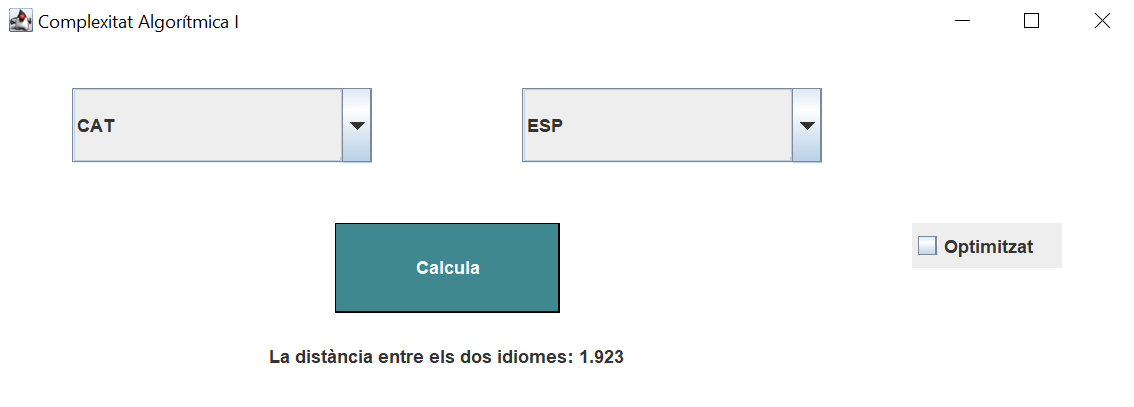
\includegraphics[width=0.4\textwidth]{images/execucio1.png}
    \caption{Resultat de l'execució 1}
\end{figure}

\subsection{Segon cas de prova}
En aquest segon cas de prova calcularem la distancia entre els idiomes francès (FRA) i anglès (ENG) utilitzant l'algorisme optimitzat. El resultat de l'execució es pot observar a la següent imatge:
\begin{figure}[ht]
    \centering
    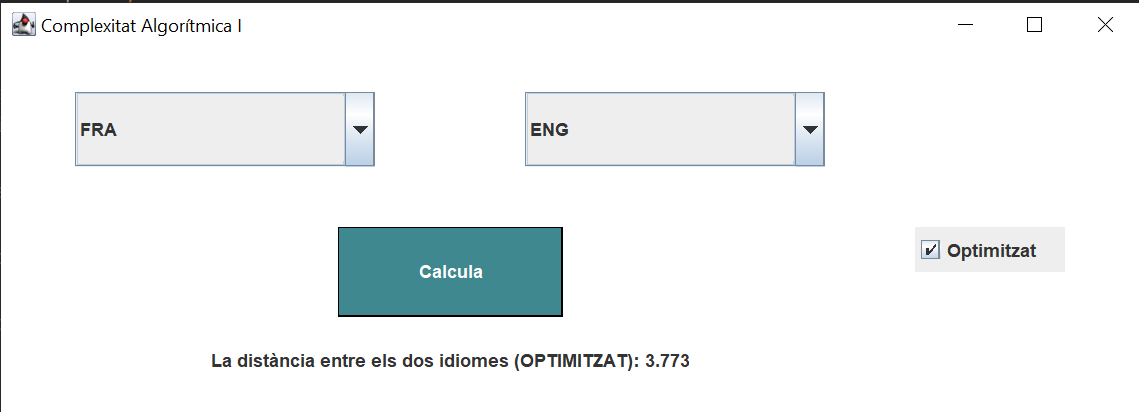
\includegraphics[width=0.4\textwidth]{images/execucio2.png}
    \caption{Resultat de l'execució 2}
\end{figure}
\subsection{Tercer cas de prova}
Per al tercer cas de prova calcularem la distancia entre els idiomes norueg (NOR) i el suec (SWE) utilitzant l'algorisme sense optimitzar. El resultat de l'execució es pot observar a la següent imatge:
\begin{figure}[ht]
    \centering
    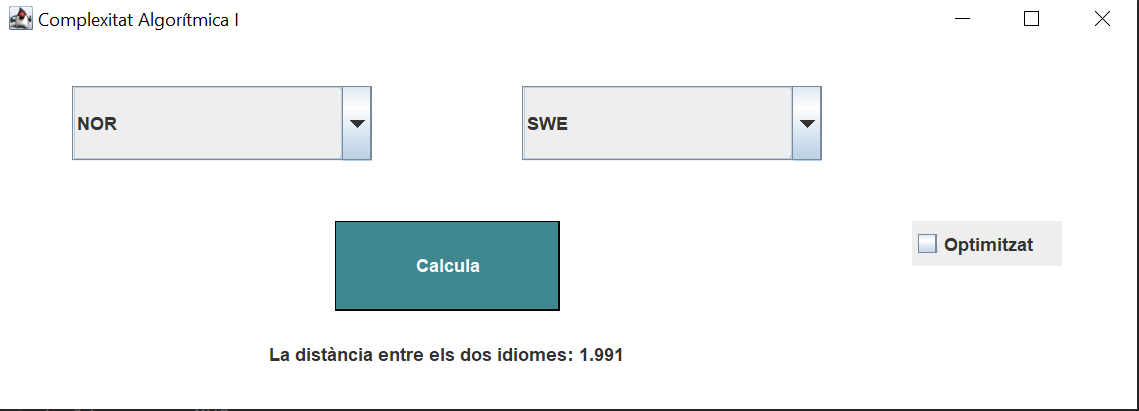
\includegraphics[width=0.4\textwidth]{images/execucio3.png}
    \caption{Resultat de l'execució 3}
\end{figure}
\subsection{Quart cas de prova}
En el cas del quart cas de prova calcularem la distancia entre els idiomes norueg (NOR) i l'italià (ITA) utilitzant l'algorisme optimitzat. El resultat de l'execució es pot observar a la següent imatge:
\begin{figure}[ht]
    \centering
    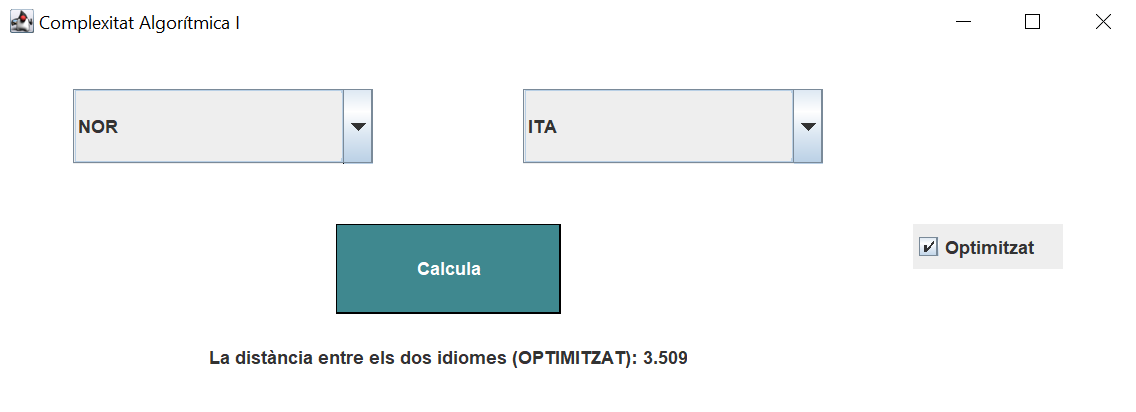
\includegraphics[width=0.4\textwidth]{images/execucio4.png}
    \caption{Resultat de l'execució 4}
\end{figure}
\subsection{Cinquè cas de prova}
Finalment, farem una execució on es calculi l distancia entre una llengua i la resta. En aquest cinquè cas de prova calcularem la distancia entre el català (CAT) i la resta de llengues. El resultat de l'execució es pot observar a la següent imatge, on es mostra la distancia que manté el català amb la resta de llengues al pop up que mostra el programa una vegada l'algorisme acaba de calcular:
\begin{figure}[ht]
    \centering
    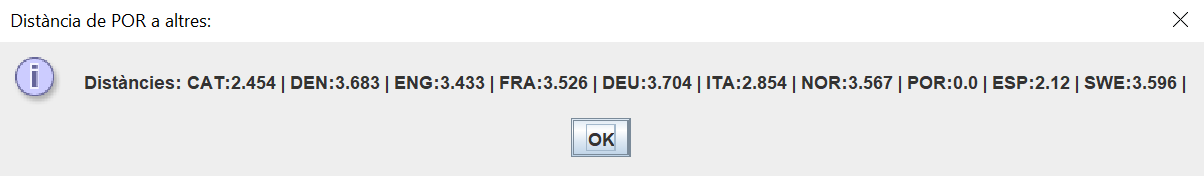
\includegraphics[width=0.4\textwidth]{images/execucio5.png}
    \caption{Resultat de l'execució 5}
\end{figure}

\section{Comparació d'algoritmes}
    En aquesta secció, ens encarregarem de comparar en termes de precisió i rendiment els dos algoritmes implementats. D'aquesta manera, hem agafat 5 execucions aleatòries i així veurem quin marge d'error s'aprecia i si el rendiment millora considerablement.\\\\ Vegem la següent taula:\\\\



\begin{table}[]
\begin{tabular}{|l|ll|ll|l|l|}
\hline
\multirow{2}{*}{} & \multicolumn{2}{l|}{No Optimitzat}     & \multicolumn{2}{l|}{Optimitzat}        & Error     & Millora   \\ \cline{2-7} 
                  & \multicolumn{1}{l|}{Valor} & Temps(ms) & \multicolumn{1}{l|}{Valor} & Temps(ms) & Valor(\%) & Temps(\%) \\ \hline
CAT-ESP           & \multicolumn{1}{l|}{1'923} & 860       & \multicolumn{1}{l|}{2'009} & 396       & 4'47      & 117'17    \\ \hline
DEU-ITA           & \multicolumn{1}{l|}{3'671} & 30.417    & \multicolumn{1}{l|}{3'711} & 14.142    & 1'09      & 115'29    \\ \hline
NOR-POR           & \multicolumn{1}{l|}{3'554} & 7.141     & \multicolumn{1}{l|}{3'567} & 5.663     & 0'37      & 26'15     \\ \hline
DEN-NOR           & \multicolumn{1}{l|}{1'142} & 3.958     & \multicolumn{1}{l|}{1'21}  & 1.353     & 5'95      & 192'31    \\ \hline
SWE-FRA           & \multicolumn{1}{l|}{3'929} & 25.156    & \multicolumn{1}{l|}{4'001} & 11.334    & 1'83      & 121'89    \\ \hline
\end{tabular}
\end{table} 

Les fórmules amb que s'han calculat l'error i la millora són les següents:\\\\
\begin{equation}
Error = \frac{|V_A-V_B|}{V_A}
\label{eq:error}
\end{equation}

\begin{equation}
Millora = (\frac{T_A}{T_B}-1) \times 100
\label{eq:acceleration}
\end{equation}

    Les variables $X_A$ corresponen als valors de l'algoritme no optimitzat, mentre que $X_B$ corresponen a valors de l'altre algoritme optimitzat.Els resultats signifiquen el següent:\\

    \begin{itemize}
        \item \textbf{Error}: el resultat s'allunya el \% determinat de la solució de l'algoritme no optimitzat. Per exemple, si el resultat bo és 100 i ens ha donat 105, tenim un marge d'error del 5\%.

        \item \textbf{Millora}: el resultat s'ha calculat un \% més ràpid amb l'algoritme optimitzat.Per exemple: un 100\% més ràpid significa que ha tardat la mitat i que és dues vegades millor que l'altre.
        
    \end{itemize}

    Si volem obtenir una mesura més uniforme, ja que tenim valors que canvien molt entre ells, realitzarem la mitjana aritmètica. Hem obtingut els resultats següents:

    $$\bar{\epsilon}=2.742\%$$
    $$\bar{\delta}=114.56\%$$

    En conclusió tenim un algoritme que tan sols s'equivoca en un $2.742\%$ de mitja i que és un $114.56\%$ més ràpid, és a dir, que tarda menys de la meitat. Realment és un sacrifici de una petita porció de precisió per un augment molt considerable en el rendiment. Cal destacar que aquest error el provoca el fet de que certs casos no són observats i si ens fixam, el valor sempre tendeix a augmentar en el cas del nostre algoritme. Per tant, suposam que el segon algoritme no contempla certs casos on la distància realment és inferior del que es troba. Finalment, aquests casos que no contempla amb distàncies majors de les originals, es va concatenant i afecta en un percentatge petit degut a la mitjana.
    



\section{Conclusions Finals}
    D'aquesta pràctica podem extreure conclusions molt interessants. En primer lloc, cal destacar que, malgrat ser més ràpid l'algoritme optimitzat, existeix un petit error. La pregunta és, val la pena la millora de \textit{performance}, sacrificant aquest càlcul més certer amb una imprecisió?\\\\

    

    La resposta, com és clar, és sí. En el cas del nostre projecte, el error no repercuteix greument sobre cap factor concret, és a dir, que un error no podria posar en risc la integritat de qualssevol. Si estiguessim en un cas on la precisió és un factor molt important, hauríem de considerar la altra possibilitat. Tot i això, existeix el dilema de que encara que sigui més certer el primer algoritme, hi ha factors externs que podrien alterar el benefici obtingut. Anem a posar un exemple: si tenim un algoritme que tarda un any i falla molt menys que un que tarda minuts, utilitzaríem el de minuts ja que en un any d'execució poden passar moltes coses a nivell de maquinari com caigudes, etc.\\\\

    Un altre factor a tenir en compte és la heurística que s'ha aplicat per veure la diferència entre dos idiomes:\\

    $$dif=\sqrt{(mean_1)^2+(mean_2)^2}$$

    Aquesta ha estat enginy per part del professor i cal destacar que és útil per a aconseguir que la distància entre dos idiomes no depengui de l'origen, és a dir, que sigui la mateixa distància $A\rightarrow B$ i $B\rightarrow A$. Això ens permet tenir un criteri més correcte i poder definir una uniformitat en els càlculs.\\\\

    Finalment,



    EXTREURE ERROR:

\section{Bibliografia}

    
\href{https://youtu.be/fwJjpH5_WDg}{Video Explicatiu de la Pràctica amb execucions}

\end{document}
